%%%%%%%%%%%%%%%%%%%%%%%%%%%%%%%%%%%%%%%%%
% Journal Article
% Data Structures and Algorithm
% Practical 3: Determine optimal window size for the Ethernet based host
%
% Gahan M. Saraiya
% 18MCEC10
%
%%%%%%%%%%%%%%%%%%%%%%%%%%%%%%%%%%%%%%%%%
%----------------------------------------------------------------------------------------
%       PACKAGES AND OTHER DOCUMENT CONFIGURATIONS
%----------------------------------------------------------------------------------------
\documentclass[paper=letter, fontsize=12pt]{article}
\usepackage[english]{babel} % English language/hyphenation
\usepackage{amsmath,amsfonts,amsthm} % Math packages
\usepackage[utf8]{inputenc}
\usepackage{float}
\usepackage{lipsum} % Package to generate dummy text throughout this template
\usepackage{blindtext}
\usepackage{graphicx} 
\usepackage{caption}
\usepackage{subcaption}
\usepackage[sc]{mathpazo} % Use the Palatino font
\usepackage[T1]{fontenc} % Use 8-bit encoding that has 256 glyphs
\usepackage{bbding}  % to use custom itemize font
\linespread{1.05} % Line spacing - Palatino needs more space between lines
\usepackage{microtype} % Slightly tweak font spacing for aesthetics
\usepackage[hmarginratio=1:1,top=32mm,columnsep=20pt]{geometry} % Document margins
\usepackage{multicol} % Used for the two-column layout of the document
%\usepackage[hang, small,labelfont=bf,up,textfont=it,up]{caption} % Custom captions under/above floats in tables or figures
\usepackage{booktabs} % Horizontal rules in tables
\usepackage{float} % Required for tables and figures in the multi-column environment - they need to be placed in specific locations with the [H] (e.g. \begin{table}[H])
\usepackage{hyperref} % For hyperlinks in the PDF
\usepackage{lettrine} % The lettrine is the first enlarged letter at the beginning of the text
\usepackage{paralist} % Used for the compactitem environment which makes bullet points with less space between them
\usepackage{abstract} % Allows abstract customization
\renewcommand{\abstractnamefont}{\normalfont\bfseries} % Set the "Abstract" text to bold
\renewcommand{\abstracttextfont}{\normalfont\small\itshape} % Set the abstract itself to small italic text
\usepackage{titlesec} % Allows customization of titles

\renewcommand\thesection{\Roman{section}} % Roman numerals for the sections
\renewcommand\thesubsection{\Roman{subsection}} % Roman numerals for subsections

\titleformat{\section}[block]{\large\scshape\centering}{\thesection.}{1em}{} % Change the look of the section titles
\titleformat{\subsection}[block]{\large}{\thesubsection.}{1em}{} % Change the look of the section titles
\newcommand{\horrule}[1]{\rule{\linewidth}{#1}} % Create horizontal rule command with 1 argument of height
\usepackage{fancyhdr} % Headers and footers
\pagestyle{fancy} % All pages have headers and footers
\fancyhead{} % Blank out the default header
\fancyfoot{} % Blank out the default footer


%----------------------------------------------------------------------------------------
%----------------------------------------------------------------------------------------
%       CUSTOM HEADER TEXT
%----------------------------------------------------------------------------------------
\fancyhead[C]{Institute of Technology, Nirma University $\bullet$ September 2018} % Custom header text
%----------------------------------------------------------------------------------------

\fancyfoot[RO,LE]{\thepage} % Custom footer text
%----------------------------------------------------------------------------------------
%       PACKAGE for code highlight
%----------------------------------------------------------------------------------------
\usepackage[utf8]{inputenc}
\usepackage[english]{babel}

\usepackage{minted} % for highlighting code sytax
%----------------------------------------------------------------------------------------
%       TITLE SECTION
%----------------------------------------------------------------------------------------
\title{\vspace{-15mm}\fontsize{24pt}{10pt}\selectfont\textbf{
		\underline{Practical 3}\\Determine optimal window size for the Ethernet based host}} % Article title
\author{\large{\textsc{
		Gahan M. Saraiya, 18MCEC10 }}\\[2mm]
%\thanks{A thank you or further information}\\ % Your name
\normalsize \href{mailto:18mcec10@nirmauni.ac.in}{18mcec10@nirmauni.ac.in}\\[2mm] % Your email address
}
\date{}
\hypersetup{
	colorlinks=true,
	linkcolor=blue,
	filecolor=magenta,      
	urlcolor=cyan,
	pdfauthor={Gahan M. Saraiya},
	pdfcreator={Gahan M. Saraiya},
	pdfproducer={Gahan M. Saraiya},
}
%----------------------------------------------------------------------------------------

\begin{document}
\maketitle % Insert title
\thispagestyle{fancy} % All pages have headers and footers

\newcommand*\tick{\item[\Checkmark]}
\newcommand*\arrow{\item[$\Rightarrow$]}
\newcommand*\fail{\item[\XSolidBrush]}

\section{Introduction}
\paragraph{}
Aim of this experiment is to determine optimal window size after which throughput saturates for ethernet based host situated nearby.

\section{Implementation}
Experiment is carried out using \textbf{iperf3} module

\subsection*{Client Reading}
\begin{minted}{text}
	iperf3 -c <server-ip-address> -w <window-size>
\end{minted}
\begin{itemize}
	\item server-ip-address here is \textit{10.1.3.34}
	\item window-size is specified in kilobytes or megabytes
\end{itemize}
Related output result are shown as below:

\inputminted[frame=lines, breaklines, linenos]{c}{../throughput_client_to_10.1.3.34.csv}

\begin{figure}[H]
	\centering
	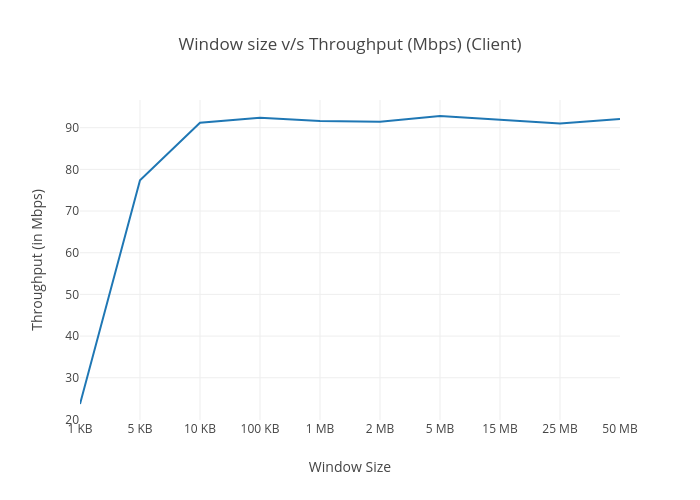
\includegraphics[scale=0.5]{../client.png}
	\caption{Graph for client measuring througput with different window sizes}
\end{figure}


\subsection*{Server Reading}
\textbf{Server IP Address}: \textit{10.1.3.34}
\\ below command will start iperf server on default port 5201
\begin{minted}{text}
	iperf3 -s
\end{minted}


Related output result are shown as below:
\inputminted[frame=lines, breaklines, linenos]{c}{../server_10.1.3.34_data.csv}

\begin{figure}[H]
	\centering
	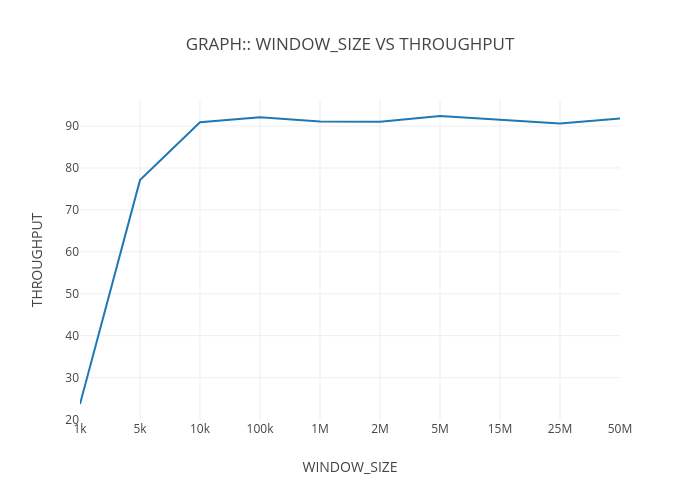
\includegraphics[scale=0.5]{../server.png}
	\caption{Graph for server througput on client request with different windows sizes}
\end{figure}

\section{Summary}
\paragraph{} As observed in above result graph increasing window size gradually increases througput till windows size reaches to \textit{10 KB} after which throughput saturates at $\approx91 Mbits/sec$.

Hence the conclusion of this experiment to determine optimal window size is achieved and it is \textit{10 KB}.

%----------------------------------------------------------------------------------------
%\end{multicols}
\end{document}
